\documentclass[11pt, a4paper]{article}
\usepackage{pdfpages}
\usepackage{parallel}
\usepackage[T2A]{fontenc}
\usepackage{ucs}
\usepackage[utf8x]{inputenc}
\usepackage[polish,english,russian]{babel}
\usepackage{hyperref}
\usepackage{rotating}
\usepackage[inner=2cm,top=1.8cm,outer=2cm,bottom=2.3cm,nohead]{geometry}
\usepackage{listings}
\usepackage{graphicx}
\usepackage{wrapfig}
\usepackage{longtable}
\usepackage{indentfirst}
\usepackage{array}
\usepackage{tikzsymbols}
\usepackage{soul}
\usepackage[ruled,vlined]{algorithm2e}
%\counterwithout{figure}{section} 

\usepackage{url}
\makeatletter
\g@addto@macro{\UrlBreaks}{\UrlOrds}
\makeatother

\newcolumntype{P}[1]{>{\raggedright\arraybackslash}p{#1}}
\frenchspacing
\usepackage{fixltx2e} %text sub- and superscripts
\usepackage{icomma} % коскі ў матэматычным рэжыме
\PreloadUnicodePage{4}

\newcommand{\longpage}{\enlargethispage{\baselineskip}}
\newcommand{\shortpage}{\enlargethispage{-\baselineskip}}

\def\switchlang#1{\expandafter\csname switchlang#1\endcsname}
\def\switchlangbe{
\let\saverefname=\refname%
\def\refname{Літаратура}%
\def\figurename{Іл.}%
}
\def\switchlangen{
\let\saverefname=\refname%
\def\refname{References}%
\def\figurename{Fig.}%
}
\def\switchlangru{
\let\saverefname=\refname%
\let\savefigurename=\figurename%
\def\refname{Литература}%
\def\figurename{Рис.}%
}

\hyphenation{admi-ni-stra-tive}
\hyphenation{ex-pe-ri-ence}
\hyphenation{fle-xi-bi-li-ty}
\hyphenation{Py-thon}
\hyphenation{ma-the-ma-ti-cal}
\hyphenation{re-ported}
\hyphenation{imp-le-menta-tions}
\hyphenation{pro-vides}
\hyphenation{en-gi-neering}
\hyphenation{com-pa-ti-bi-li-ty}
\hyphenation{im-pos-sible}
\hyphenation{desk-top}
\hyphenation{elec-tro-nic}
\hyphenation{com-pa-ny}
\hyphenation{de-ve-lop-ment}
\hyphenation{de-ve-loping}
\hyphenation{de-ve-lop}
\hyphenation{da-ta-ba-se}
\hyphenation{plat-forms}
\hyphenation{or-ga-ni-za-tion}
\hyphenation{pro-gramming}
\hyphenation{in-stru-ments}
\hyphenation{Li-nux}
\hyphenation{sour-ce}
\hyphenation{en-vi-ron-ment}
\hyphenation{Te-le-pathy}
\hyphenation{Li-nux-ov-ka}
\hyphenation{Open-BSD}
\hyphenation{Free-BSD}
\hyphenation{men-ti-on-ed}
\hyphenation{app-li-ca-tion}

\def\progref!#1!{\texttt{#1}}
\renewcommand{\arraystretch}{2} %Іначай формулы ў матрыцы зліпаюцца з лініямі
\usepackage{array}

\def\interview #1 (#2), #3, #4, #5\par{

\section[#1, #3, #4]{#1 -- #3, #4}
\def\qname{LVEE}
\def\aname{#1}
\def\q ##1\par{{\noindent \bf \qname: ##1 }\par}
\def\a{{\noindent \bf \aname: } \def\qname{L}\def\aname{#2}}
}

\def\interview* #1 (#2), #3, #4, #5\par{

\section*{#1\\{\small\rm #3, #4. #5}}
\ifx\ParallelWhichBox\undefined%
    \addcontentsline{toc}{section}{#1, #3, #4}%
\else%
\ifnum\ParallelWhichBox=0%
    \addcontentsline{toc}{section}{#1, #3, #4}%
\fi\fi%

\def\qname{LVEE}
\def\aname{#1}
\def\q ##1\par{{\noindent \bf \qname: ##1 }\par}
\def\a{{\noindent \bf \aname: } \def\qname{L}\def\aname{#2}}
}

\newcommand{\interviewfooter}[1]{
\vskip 1em
\noindent \textit{#1}
}

\switchlang{ru}
\begin{document}

\title{1983 "--- Apple Lisa mouse}
\date{}
\maketitle
\selectlanguage{russian}
Мышь для компьютеров Apple Lisa была выпущена в 1983 году \cite{mouses} и считается одной из первых компьютерных мышей, доступных в свободной продаже (рис. \ref{fig:AppleLisaPic}).

\begin{figure}[h]
   \centering
    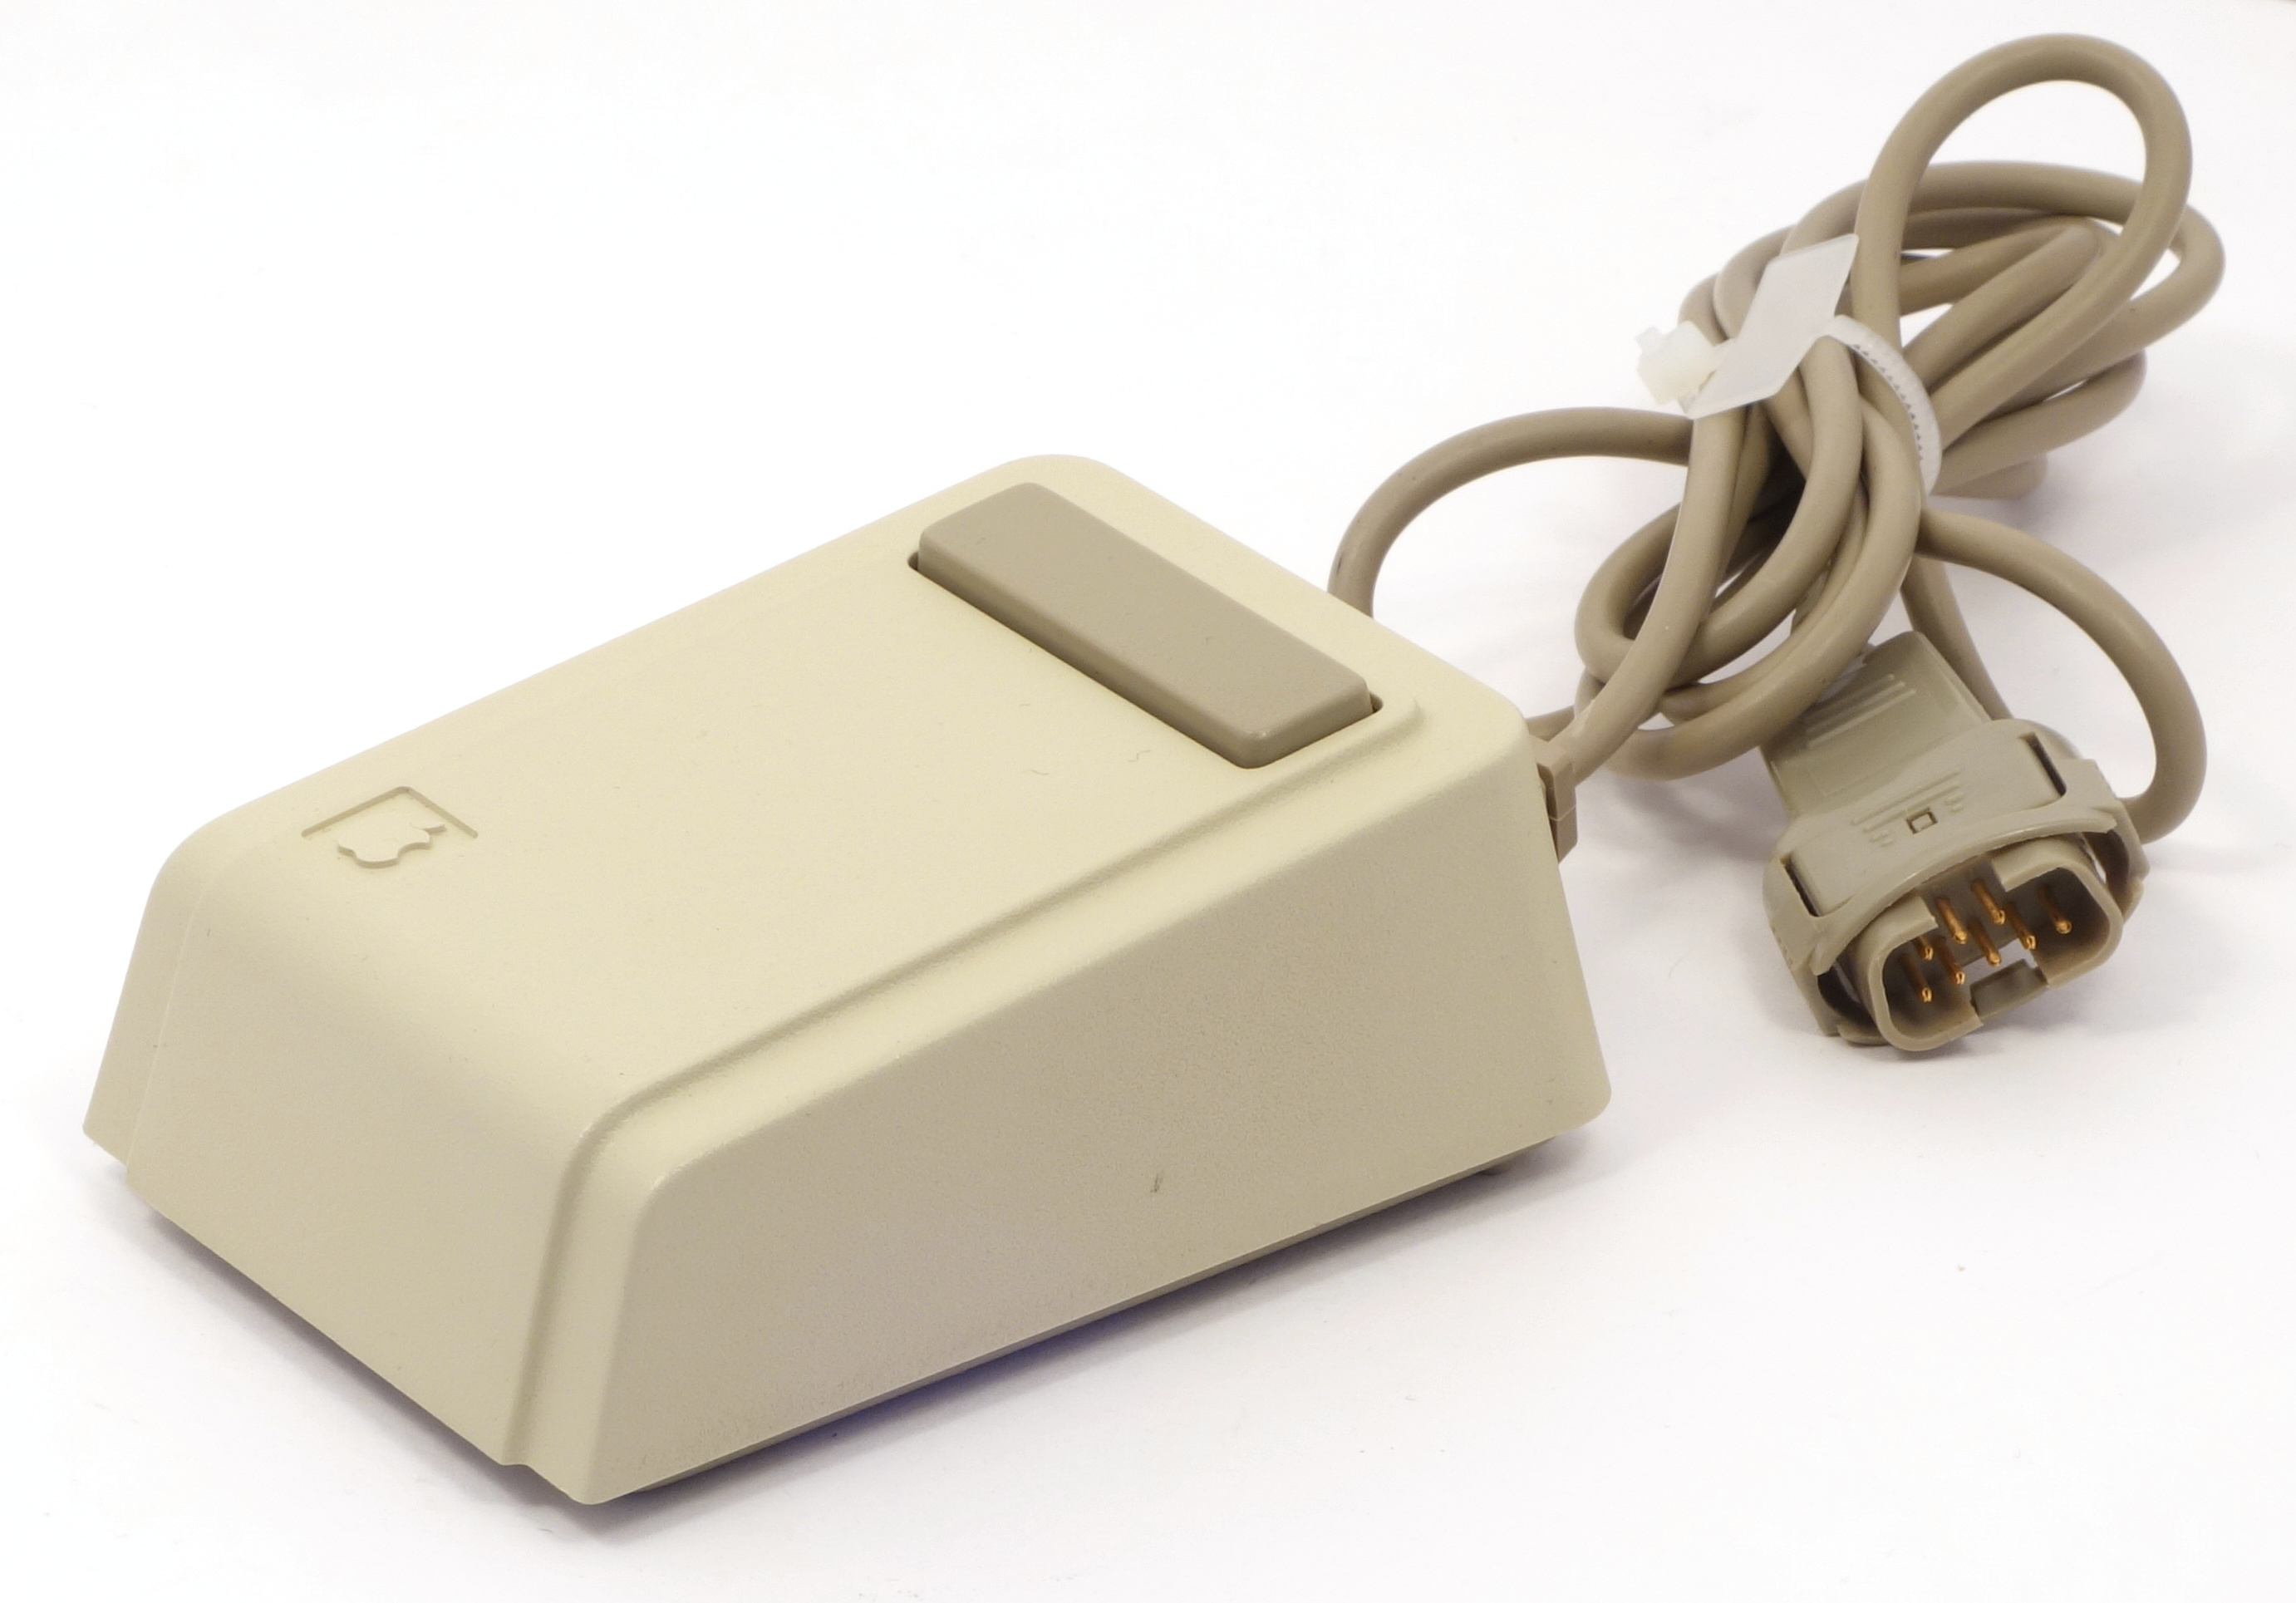
\includegraphics[scale=0.5]{1983_apple_lisa_mouse/applenorm_30.jpg}
    \caption{Apple Lisa mouse, вид спереди}
    \label{fig:AppleLisaPic}
\end{figure}

Мышь производилась Apple, но авторство ее разработки принадлежит сторонней компании Hovey-Kelley (позже переименованной в IDEO). Отталкиваясь от дизайна мышей Xerox и Hawley Mouse House, команда разработчиков создала более дешевую и при этом лучшую в техническом плане механическую часть, и разработала сложную внутреннюю конструкцию корпуса, удерживающую ее части вместе. Большое внимание было уделено и другим ключевым компонентам мыши, вплоть до акустических и тактильных особенностей нажатия кнопки и прорезиненного покрытия на шарике \cite{ideo}.

\begin{figure}[h]
    \centering
    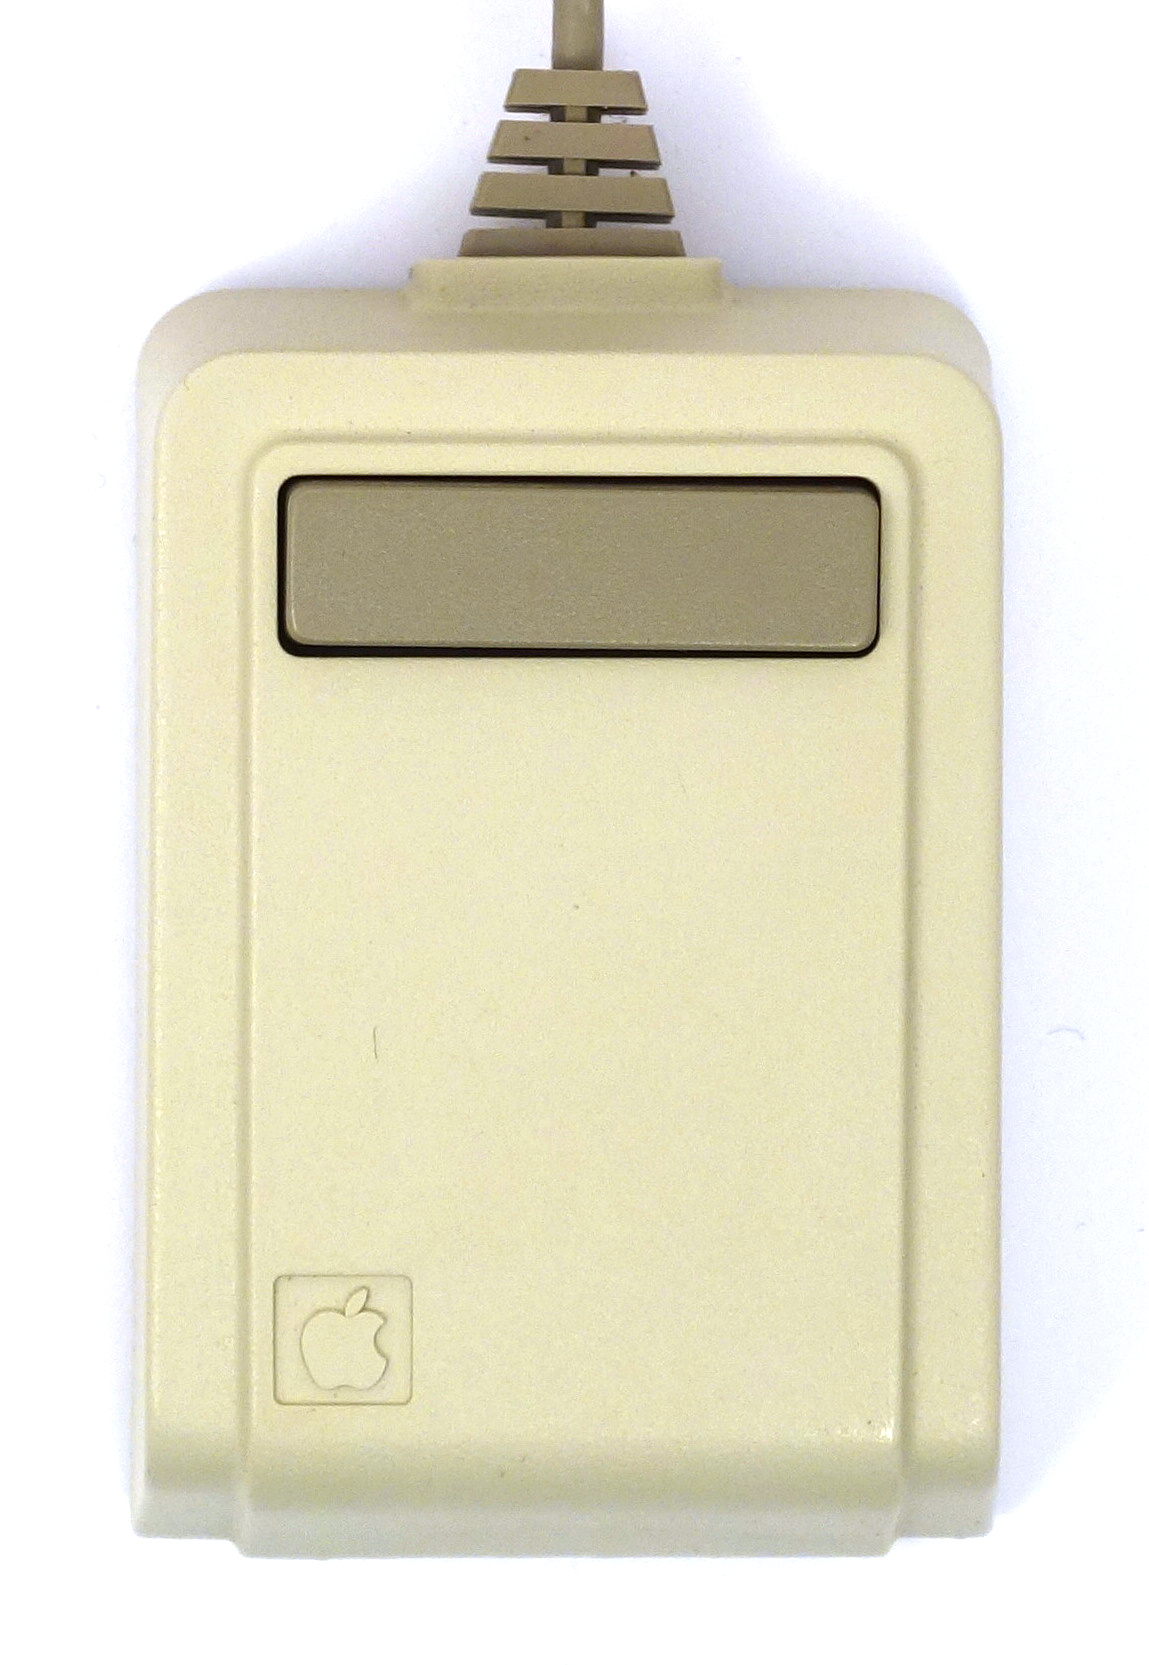
\includegraphics[scale=0.5]{1983_apple_lisa_mouse/appletop_60.jpg}
    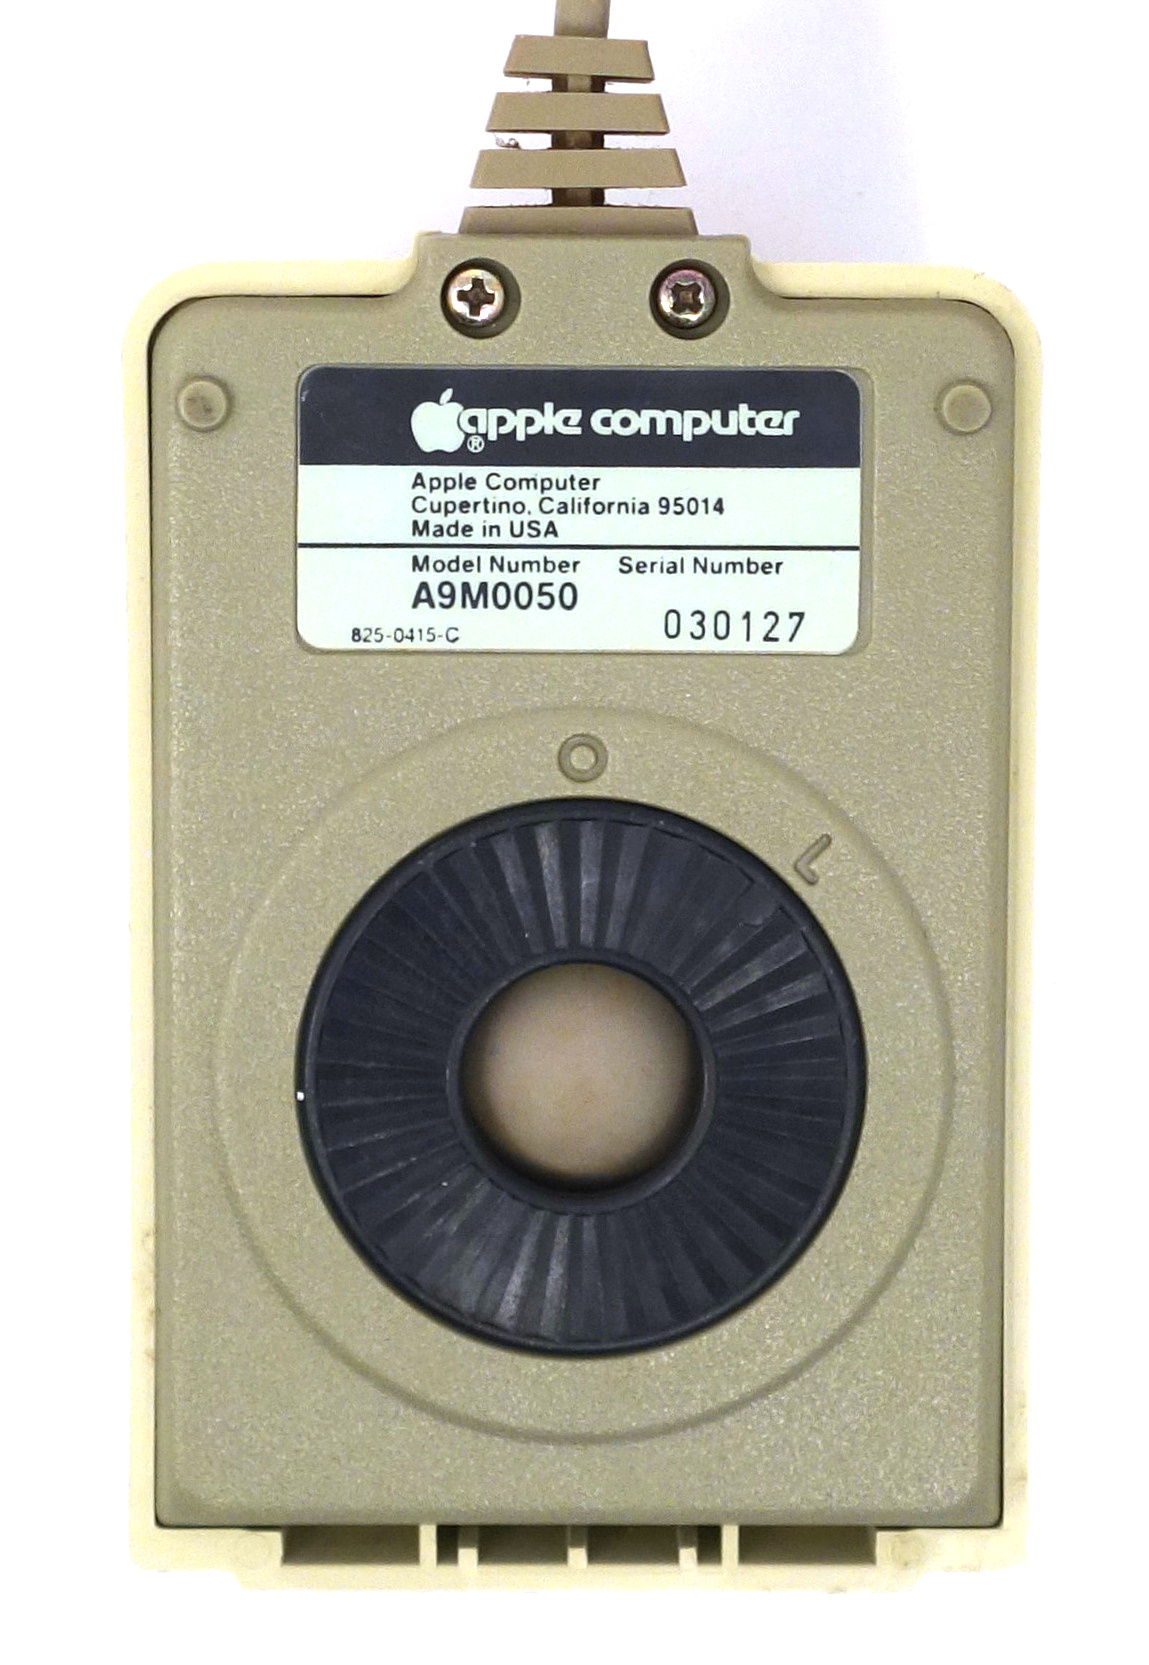
\includegraphics[scale=0.5]{1983_apple_lisa_mouse/applebottom_60.jpg}
    \caption{Apple Lisa mouse, вид сверху и снизу}
    \label{fig:AppleLisaTopAndBottom}
\end{figure}

Корпус мыши Lisa представляет собой наклонную коробку бежевого цвета. Нижняя стенка корпуса мыши, кабель и кнопка окрашены в коричневый цвет. На корпусе присутствует рельефный логотип Apple (рис. \ref{fig:AppleLisaTopAndBottom}). Шар выполнен из металла и имеет резиновое покрытие для лучшего сцепления с поверхностью, в отличие от более ранних мышей, имевших либо резиновый либо гладкий стальной шар. В последствии подобная реализация шара, а также съёмное кольцо, позволяющее легко извлечь шар для удаления собравшегося мусора, станут стандартом. То же самое можно сказать и про базовую конструкцию ее механизма, которая в дальнейшем использовалась в абсолютном большинстве оптомеханических мышах.

\begin{figure}[h]
    \centering
    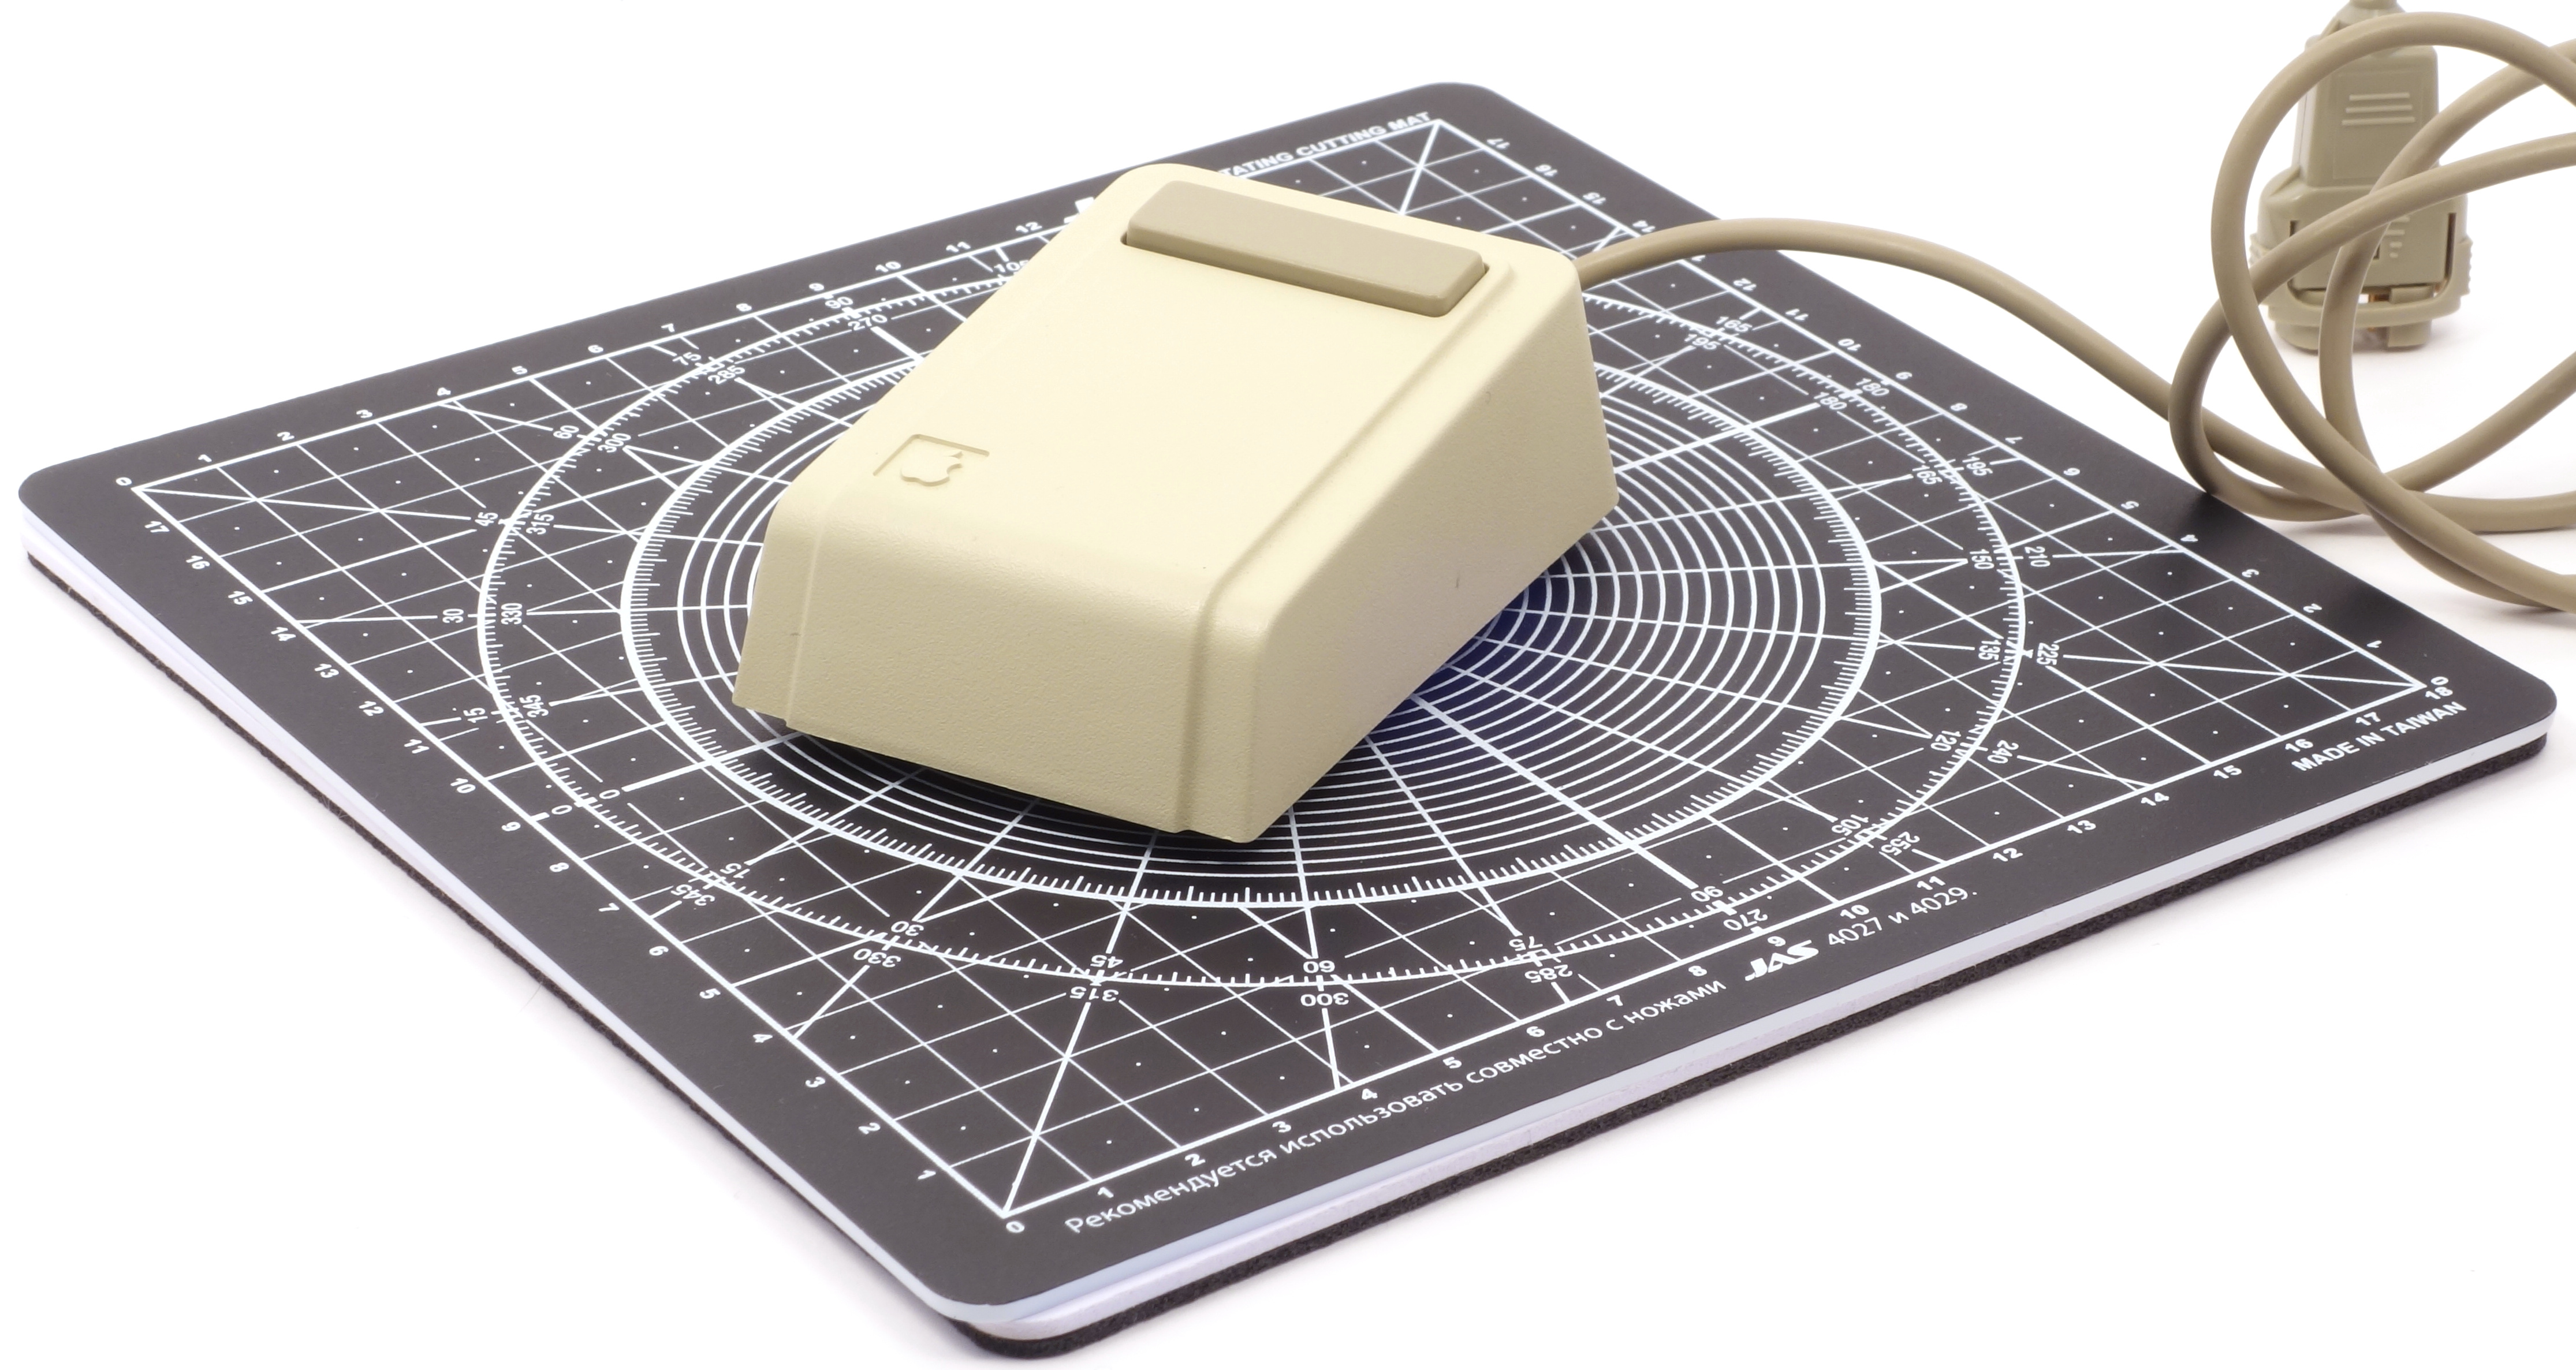
\includegraphics[scale=0.4]{1983_apple_lisa_mouse/applekovrik_60.jpg}
    \caption{Apple Lisa I на размерном коврике с шагом сетки 1~см}
    \label{fig:AppleLisaSize}
\end{figure}

Несмотря на то, что мышь имеет сравнительно небольшие размеры, впрочем, характерные для мышей 1980-х годов (рис. \ref{fig:AppleLisaSize}), исследования ее разработчиков не прошли даром, и она достаточно удобно лежит в руке. При этом единтвенная кнопка расположена ортогонально кабелю и рассчитана на нажатие скорее двумя пальцами, чем одним (рис. \ref{fig:AppleLisaHand}), а тактильность нажатия обеспечивается специально предусмотренным пружинным механизмом.

\begin{figure}[h]
    \centering
    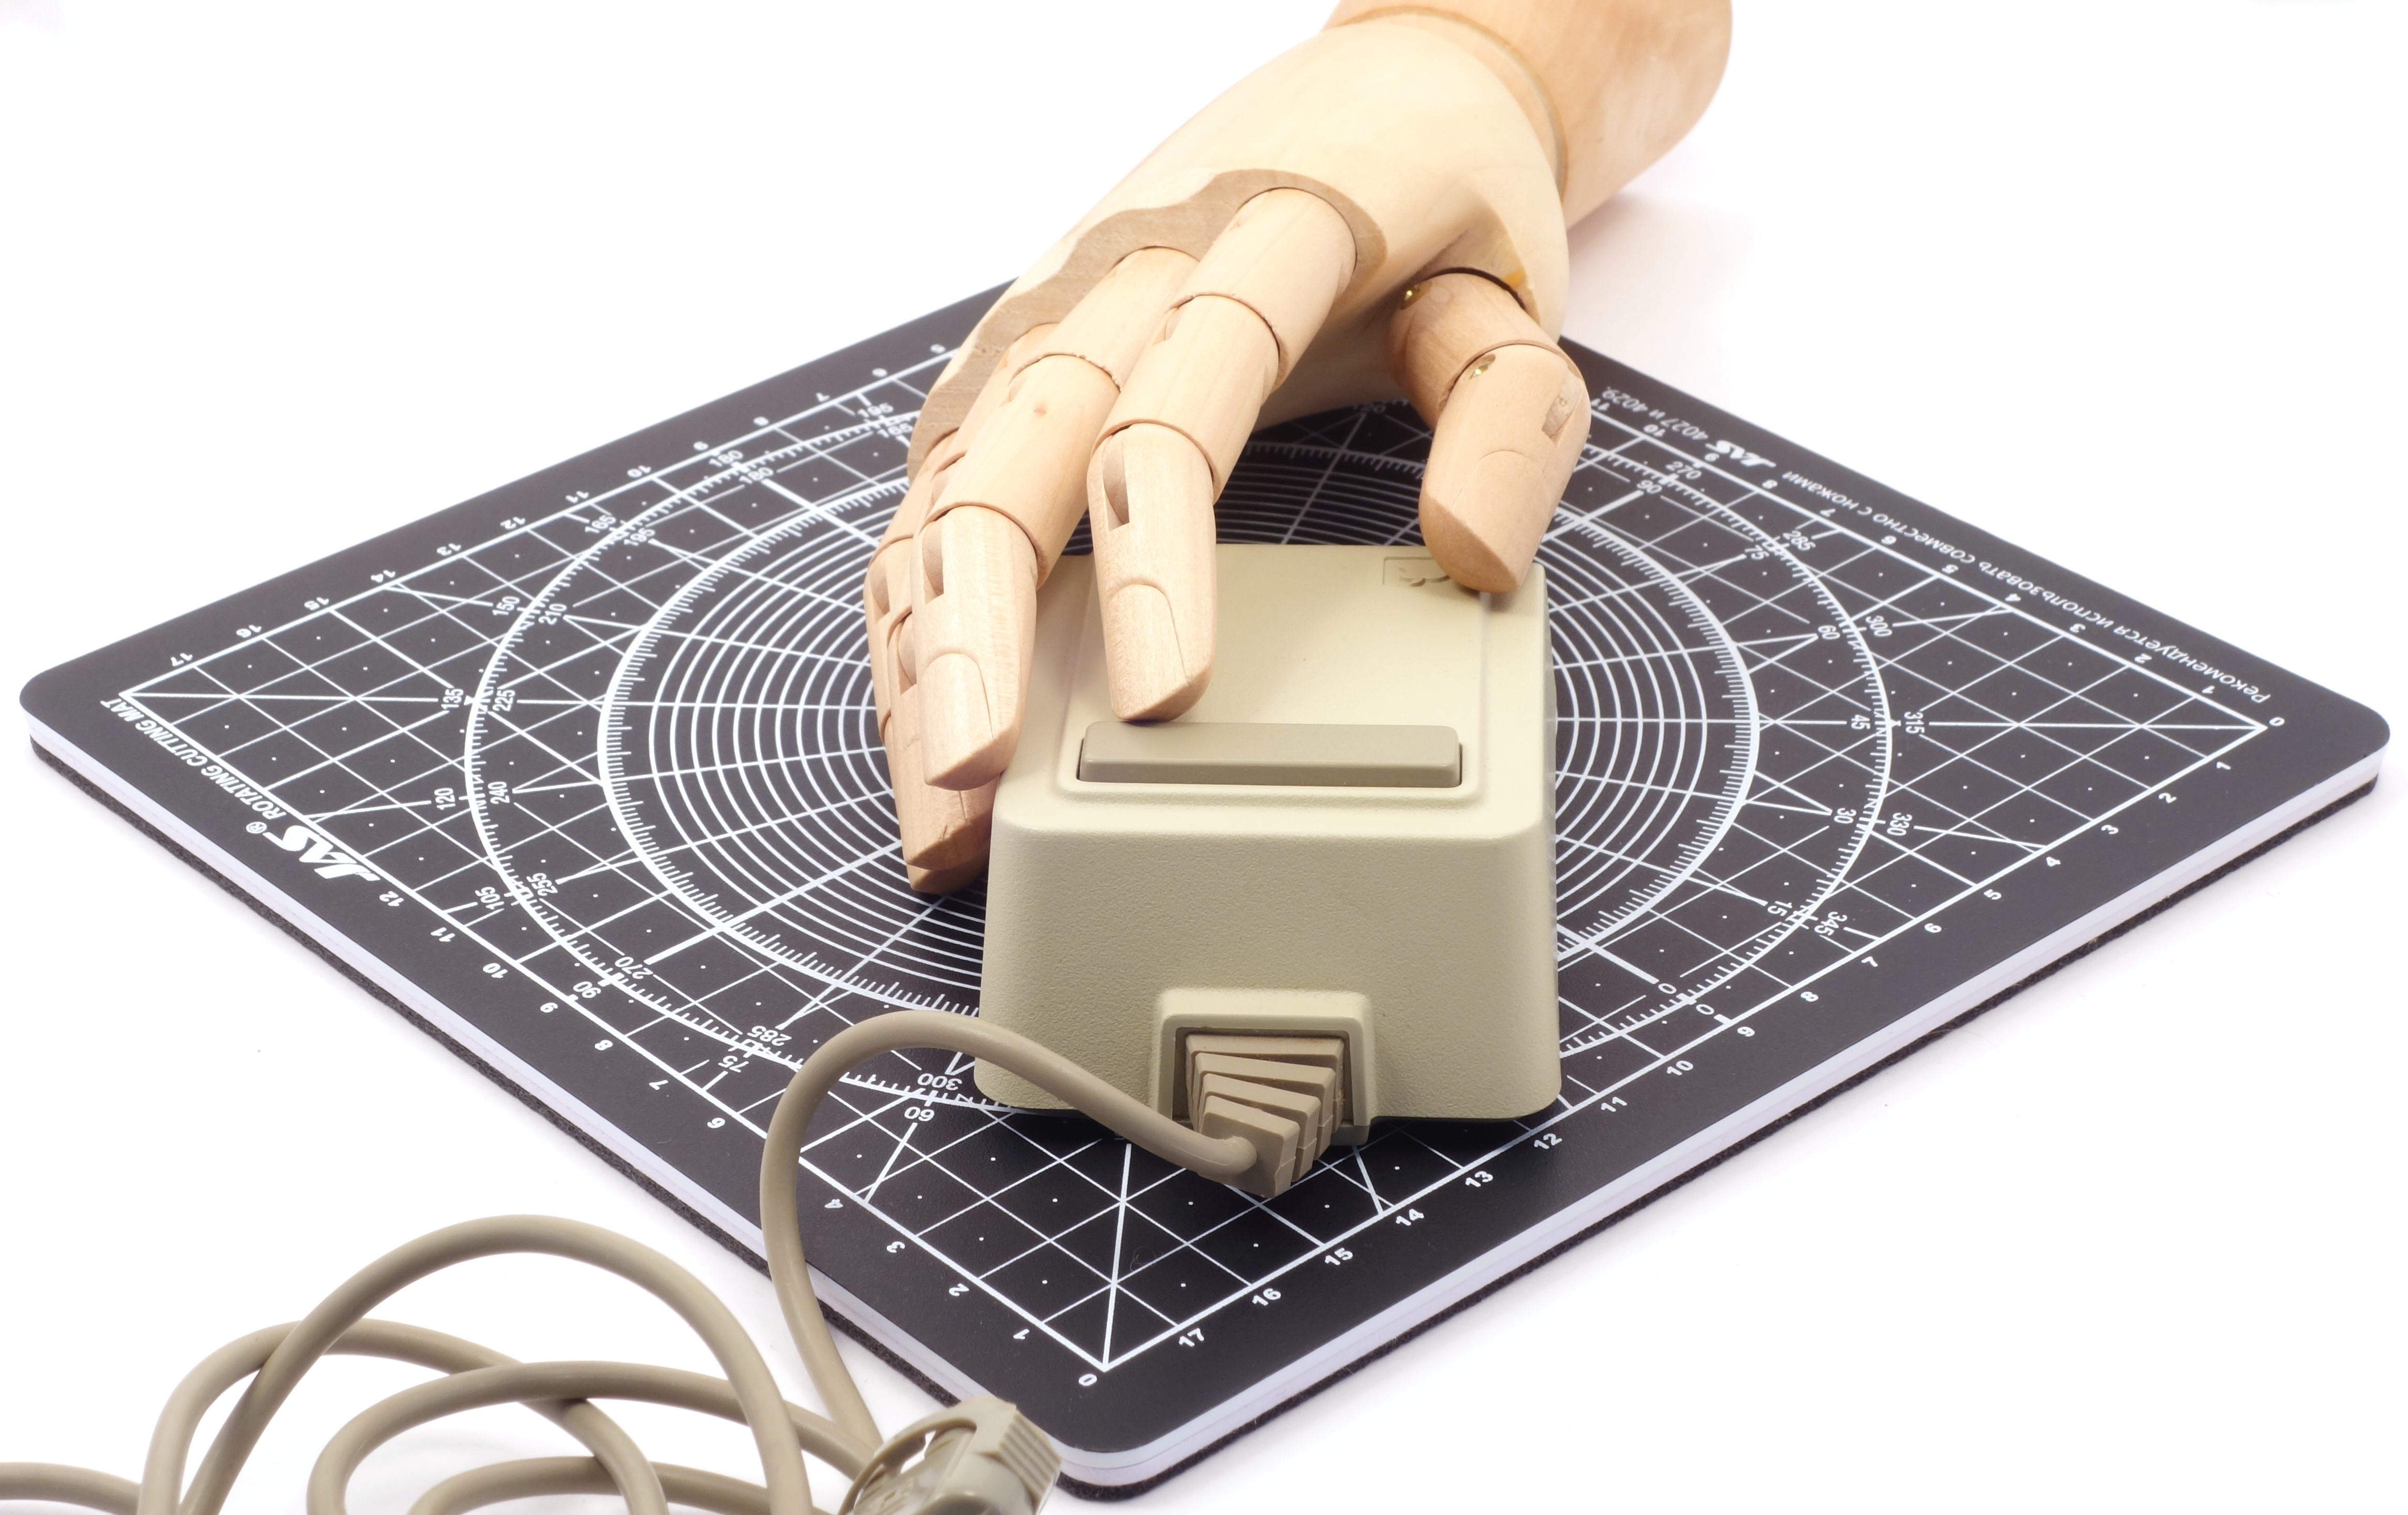
\includegraphics[scale=0.4]{1983_apple_lisa_mouse/appleruka_60.jpg}
    \caption{Apple Lisa I с моделью руки человека}
    \label{fig:AppleLisaHand}
\end{figure}

Внутреннее устройство мыши показано на рис. \ref{fig:AppleLisaInside}. Можно отметить достаточно сложную внутреннюю конструкцию корпуса со значительным числом перегородок и дополнительных опор. Унаследовав конструкцию оптомеханическуого энкодера практически без изменений, производители последующих мышей постепенно все более упрощали внутреннюю конструкцию корпуса, достигнув к девяностым годам практически пустотелой конструкции устройства.

 \begin{figure}[h]
    \centering
    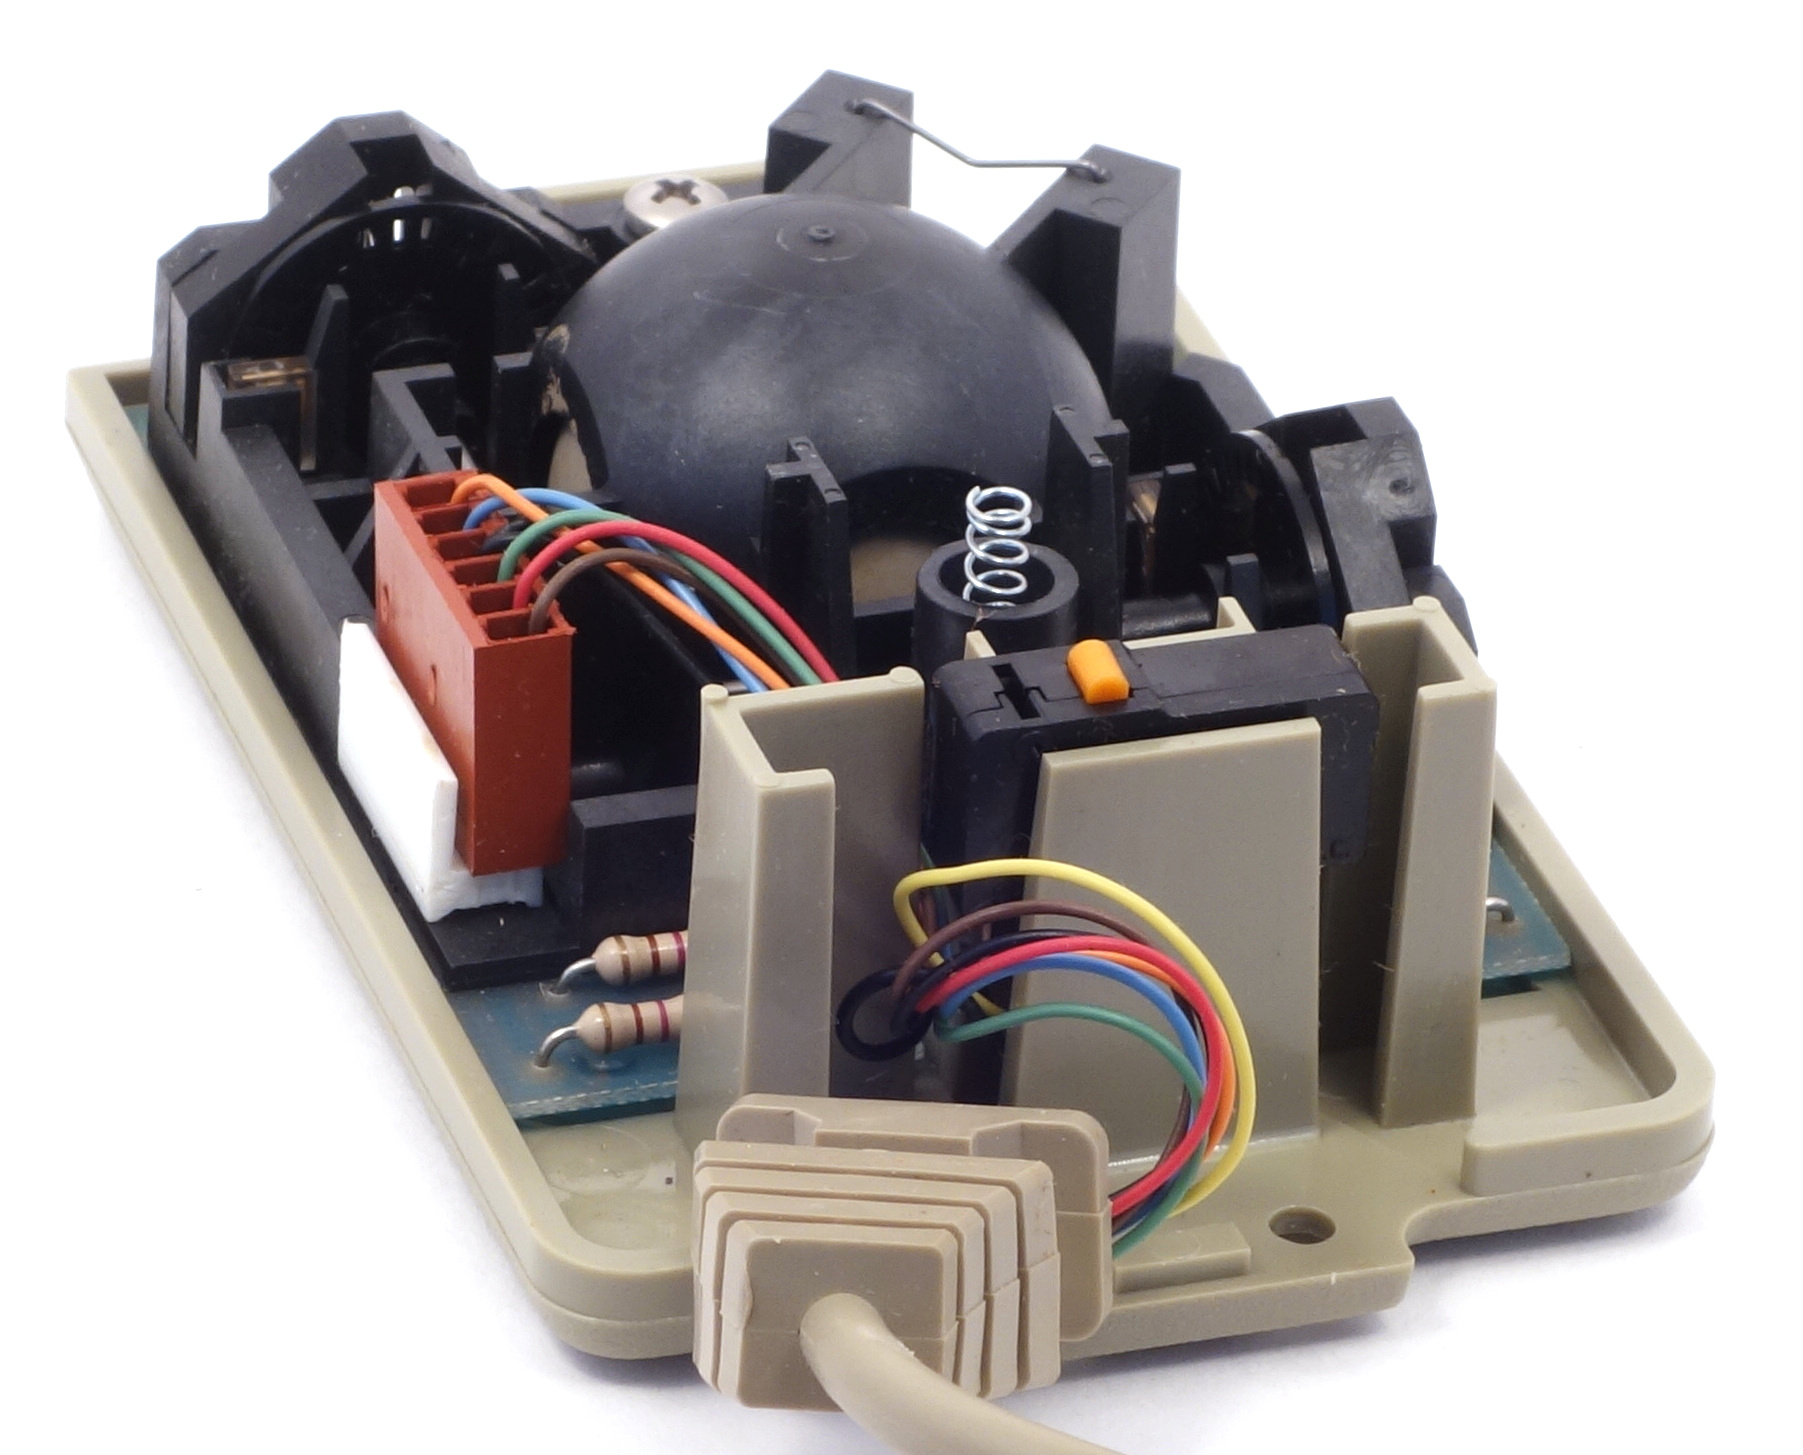
\includegraphics[scale=0.6]{1983_apple_lisa_mouse/appleraz_60.jpg}
    \caption{Apple Lisa I в разобранном виде}
    \label{fig:AppleLisaInside}
\end{figure}

\begin{thebibliography}{9}
\bibitem {mouses} Apple Lisa I Mouse \url{https://www.oldmouse.com/mouse/apple/lisa.shtml}

\bibitem {ideo} Creating the First Usable Mouse \url{https://www.ideo.com/case-study/creating-the-first-usable-mouse}
\end{thebibliography}
\end{document}
